\chapter{Rotating solar systems and radio astronomy}

\section{introduction} 
You would think that being limited to radio signals, the kinds of observations you could make and the information you could gather would be relatively small. In fact, there are a wide range of observations and interesting phenomena which can be detected using a radio telescope. From the elemental make up of a distant planet's atmosphere, to the detection of extreme astronomical objects. In fact, we can use observations of signals from hydrogen clouds in the galactic plane and, using the knowledge we gained of the Doppler shift, obtain an estimate for the distribution of matter in the Milky Way. By now you know how to go from radio signals to velocity, but how do you go from velocity to mass? In this lab, not only will you learn how we can estimate mass distribution, but you will also learn the basics of using the Small Radio Telescope. 

\section{Learning Goals}
\begin{itemize}
	\item Make predictions about large, gravitationally bound systems based on observations of smaller scale systems.
	
	\item Make observations using the Small Radio Telescope (SRT) and interpret the data
	
	\item Calibrate the SRT and understand the uncertainty by measuring background noise in the Chicago sky 
\end{itemize}

\section{Masses and Orbital Velocity} %working title only
One of the main labs you will carry out this quarter is a measurement of the motion of the Milky Way using the SRT. It is important that when you make these measurements that you understand the results you obtain. In this experiment, you will learn how the specific observations you will make can be used to make some predictions about the milky way. 

\subsection{Goal}
Learn how new phenomena can be predicted or inferred from basic physical principles and how to interpret rotation curves. 

\subsection{Equipment}

\begin{itemize}
	\item Desmos Graphing Calculator: https://www.desmos.com/calculator
\end{itemize}

\subsection{steps}

\begin{steps}
	\item First, we know from Newton's first law that the force on an object is equal to its mass times its acceleration, $F=ma$. We also know that an object moving in a circle will experience an acceleration towards the center of its path which is given by $a = \dfrac{v^2}{r}$, where $v$ is the velocity of the object and r is the radius of its path. Using these two equations, find an equation for the force experienced by an object undergoing circular motion. 
	
	\item Objects in orbit also move in an approximately circular path and the force of gravity they experience is given by $F = G\dfrac{Mm}{r^2}$, where M and $m$ are the masses of the two objects and $G$ is the gravitational constant. Using the equation you found in the previous step, derive an equation for the velocity of the orbiting object as a function of its radius.\textit{Remember to cancel out like factors. Your equation should be in terms of M, r, and G}
\end{steps}

Below you will find what is known as a \textit{rotation curve}, which plots the orbital velocities of objects in an orbital system against their distance from the center. Using these curves, it is possible to learn a lot about the system it describes. 

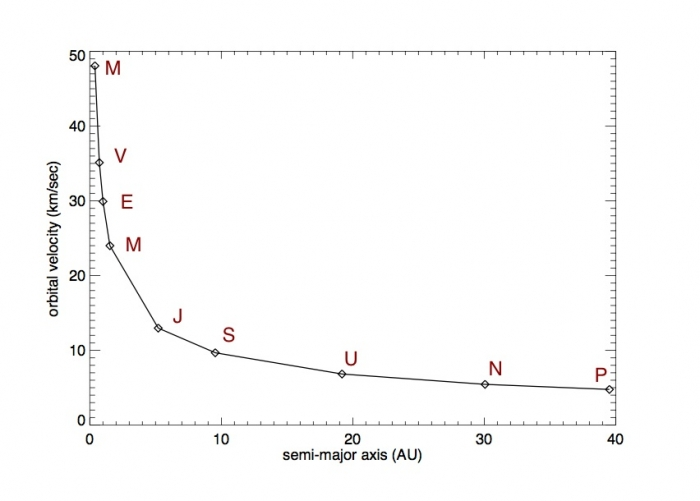
\includegraphics[scale = .7]{srt-background-rotation/keplerian-orbit.jpg}

\begin{steps}
	\item Describe the graph  that you see. How does velocity change as you move away from the center of rotation? \textbf{Write your answer in the lab report}
	
	\item This rotation curve can be modeled by the equation you found above. How would you manipulate the equation to obtain the curve. What variables would have to change? Which values would remain the same? \textit{It might help  to use the graphing calculator provided in the link above} \textbf{Write your answers down}
	
\end{steps} 

When you first derived the equation for rotational velocity, you assumed that $M$ represented the mass for a single object. Now assume that it represents the total mass contained within the orbital radius. 

\begin{steps}
	\item Given the above rotation curve, how does the mass contained change as you move farther from the center of the orbital system? Does it change? What does this tell you about the distribution of mass in the orbital system?
\end{steps}

Now we will take a look at curve B from the graph below
	
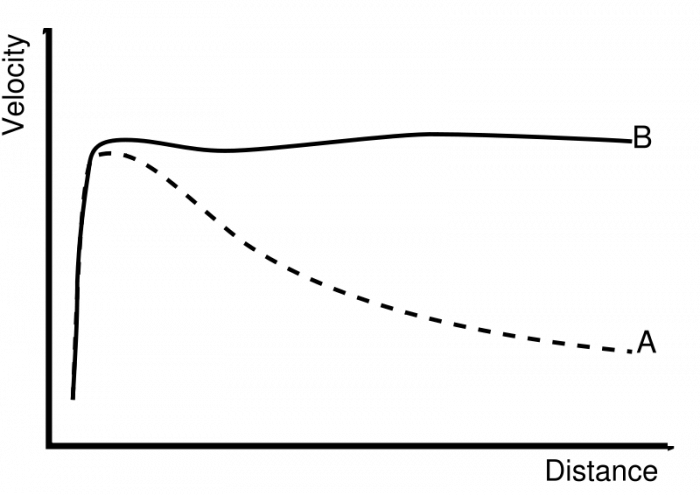
\includegraphics[scale = .5]{srt-background-rotation/galactic_rotation_curve}

\begin{steps}
	\item Following a similar process to what you used for the first curve, what changes would you have to make to obtain curve B so that velocity remains constant. \textit{Specifically, how would M have to change with respect r to make v constant}
	
	\item Based on your answer to the previous question, what does curve B tell you about the distribution of mass in the orbital system? 
	
	\item Now, look up information on the masses of the planets in the solar system as well as the sun. Which of the two rotation curves would you expect the solar system to have? \textit{It might help to add up all the masses and see how much each planet contributes to the total mass}
	
\end{steps}
	


\section{Background Noise} %working title only
While learning about the theory behind making astronomical observations is always useful, the best way to gain an intuition for these concepts is through hands on experience. For this experiment, you will learn how to operate the small radio telescope located on top of the Eckart Research Center. In particular, you will learn how to calibrate the telescope and measure the background noise present in the Chicago sky.

\subsection{Data Output} 

When using the telescope you will notice that it outputs a temperature. This is not that the SRT is actually measuring the object's temperature, rather, it is simply interpreting the power it receives as a temperature. Similarly, when calibrating, the telescope will display a system temperature $T_sys$ which interferes with our measurements. When calibrating, we account for $T_sys$ and it is subtracted from our measurements. 

\subsection{Telescope Control}
Unfortunately, you will not be able to directly control the telescope and it will instead be controlled by a designated telescope technician. However, you should still learn the basics of controlling the telescope so you can give the technician proper observation instructions. In this case, the technician will act as your hands when operating the telescope, inputting the commands you give them.

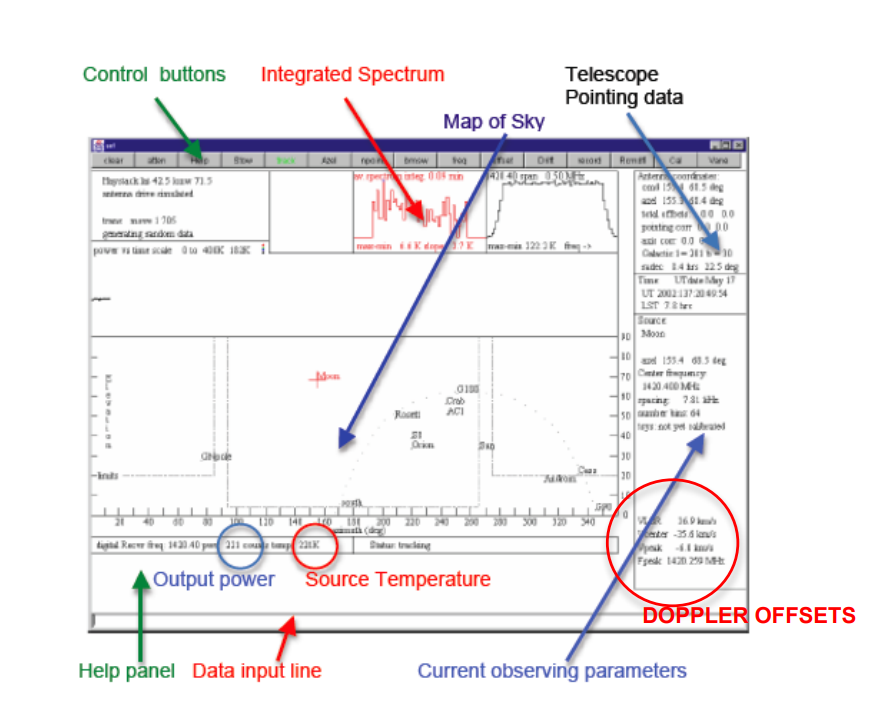
\includegraphics[scale = .9]{srt-background-rotation/display_diagram}

\subsection{Control Buttons}
The control panel display has a line of control buttons at the top that set
up a command for the telescope. For instance, if you want to change the receiver
frequency, you click on the “freq” button. Instructions and help information are
then displayed in the help panel below the map while the cursor is pointed to the
button (This field is blank when you move the cursor away). If you want to
change the frequency, then type data into the data line (e.g. “1420.4 4”), click
“enter” or “return”. Be sure you leave a space between 1420.4 (which is the
frequency) and the number 4 (which sets the bandwidth of the system). The
current observing parameters will be updated in the appropriate box.

\subsection{Control Display \& Sky Map}
The control panel shows a map of the current sky in Azimuth and
Elevation units. 0 degrees azimuth points North, 90 degrees points East, 180
degrees points South and 270 degrees points West. The horizon is at 0 degrees
elevation and Zenith is at 90 degrees. The telescope can point to about 85
degrees in elevation.
The map displays objects visible at the current time. The software tracks
an object or a given azimuth and altitude position, including corrections for the
rotation of the earth. Also displayed on the map are various individual
astronomical sources and a track of dots that show the plane of the Milky Way.
The Longitude of points along the equator of the Milky Way are shown as Gxxx,
where xxx is the Galactic longitude. We have an unobstructed view of all objects
above about 20 degrees.

\subsection{Pointing the Telescope}
You can point to any given position in the sky by clicking on the “AzEl”
button and then typing the desired Azimuth and Elevation in the command line at
the bottom of the display. (e.g., 30 45 “enter” will send the telescope to a position
of 30 degrees azimuth and 45 degrees elevation). When you enter a position you
will see a yellow cross and the CMD numbers will change to these numbers. 

When “track” shows up in green at the top of the display, the telescope has
acquired the position and is tracking it, this holds for sources. If the telescope
does not move, then you probably have to click on “track”.
Occasionally the telescope motor will get stuck and stall. Normally it fixes
itself automatically by going back to the “Stow” position (where it is stowed after
every observation), but if it remains stalled for several minutes click “Stow” to do
so manually. This can be a nuisance and time-consuming but you should still be
able to obtain the necessary data if this happens.

\subsection{Steps}
\begin{steps}
	\item Set the receiver frequency to 1416MHz. At this frequency, you will detect the continuum radiation. That is, radiation emitted relatively uniformly over a broad band of frequencies  
	
	\item Point the telescope at a position in the sky away from the galactic plane. Do this by choosing Azimuth and Elevation (AzEl) coordinates which do not lie in the arc of labeled locations on the telescope display. \textbf{Record these coordinates}
	
	\item Once the telescope has reached the given position, click ``Clear'' to erase any previous reading. Record the raw temperature displayed. Then click ``Cal'' to calibrate the telescope. \textbf{Record the new output temperature.} 
	
	\item Repeat the calibration a few times until you read a stable system temperature $T_{sys}$. Wait around 1 minute between calibrations
	
	\item After you have successfully calibrated the telescope, from you calibration position, point the telescope 15 degrees lower in elevation and calibrate the telescope 2-3 more times. \textbf{Record $T_{sky}$ and $T_{sys}$ as well as the telescope coordinates}
	
	\item Returning to your original pointing elevation, repeat the above step but this time changing the azimuth by 50 or 75 degrees.
	
	\item From your observations, how uniform is the sky in Hyde Park? \textbf{Include a table of your measurements and a discussion of the question in your report.}
\end{steps}